\subsection{Gaussian Splatting}
Przy pomocy biblioteki \textit{gsplat}\cite{ye2024gsplatopensourcelibrarygaussian} implementującej Gaussian Splatting w Pythonie wykonaliśmy eksperymenty polegające na uruchomeniu algorytmu dla różnych wartości hiperparametrów w celu znalezienia optymalnych dla nich wartości. 

\textbf{Działanie algorytmu}

Na wejściu otrzymywana jest chmura punktów uzyskana w procesie rekonstrukcji, która jest bazą do dalszego dzielenia i powstawania "gaussianów", a ich parametry: pozycja, kolor, skala i rotacja są optymalizowane przy pomocy metody spadku wzdłuż gradientu. 


\textbf{Znaczenie wartości hiperparametrów}
\begin{enumerate}
    \item Liczba Gaussianów: w przypadku scen urbanistycznych w celu oddania odpowieniej szczegółowości potrzebne jest parę milionów Gaussianów, dla naszych scen było to zwykle 3 mln.
    \item Strategia adaptacji: jej wybór jest istotny gdyż określa sposób dodawania i usuwania Gaussianów oraz wpływa na jakość sceny. Możliwe są dwa wybory: "default" i "mcmc".
    \item Częstość adaptacji: wpływa na tempo wzrostu liczby gaussianów, wybrana wartość zależy od strategii i powinna być mniejsza niż 500 dla "mcmc" i większa niż 500 dla "default"
    \item Liczba iteracji: zwykle im dłużej trenowana jest scena tym lepsze wyniki otrzymujemy, jednak zależy to również od przyjętej strategii. Liczba ta wpływa bezpośrednio na czas trenowania, powinna wynieść nie mniej niż paręnaście tysięcy.
    \item Stopień zmiennych harmonicznych: zmienne harmoniczne wyrażają kolor, im większy stopień tym lepsza jakość sceny, ale też zwiększone zużycie pamięci.  
\end{enumerate}

\textbf{Proces optymalizacji}

Głównymi metrykami przyjętymi do oceny jakości są SSIM (Structural Similarity Index Measure), PSNR (Peak Signal-to-Noise Ratio) oraz LPIPS (Learned Perceptual Image Patch Similarity). Warto podkreślić, że czas trenowania wynosi zwyklę parę godzin w zależności od przyjętych ustawień, a do procesu trenowania potrzebna jest CUDA. 

\textbf{Przykładowe wizualizacje}

Poniższe renderowania zostały wykonane przy pomocy biblioteki nerfview która również służy do wizualizacji splatów. Na poniższych rysunkach są od lewej do prawej: prawdziwe zdjęcie i widok modelu

\begin{figure}[!h]
    \centering
    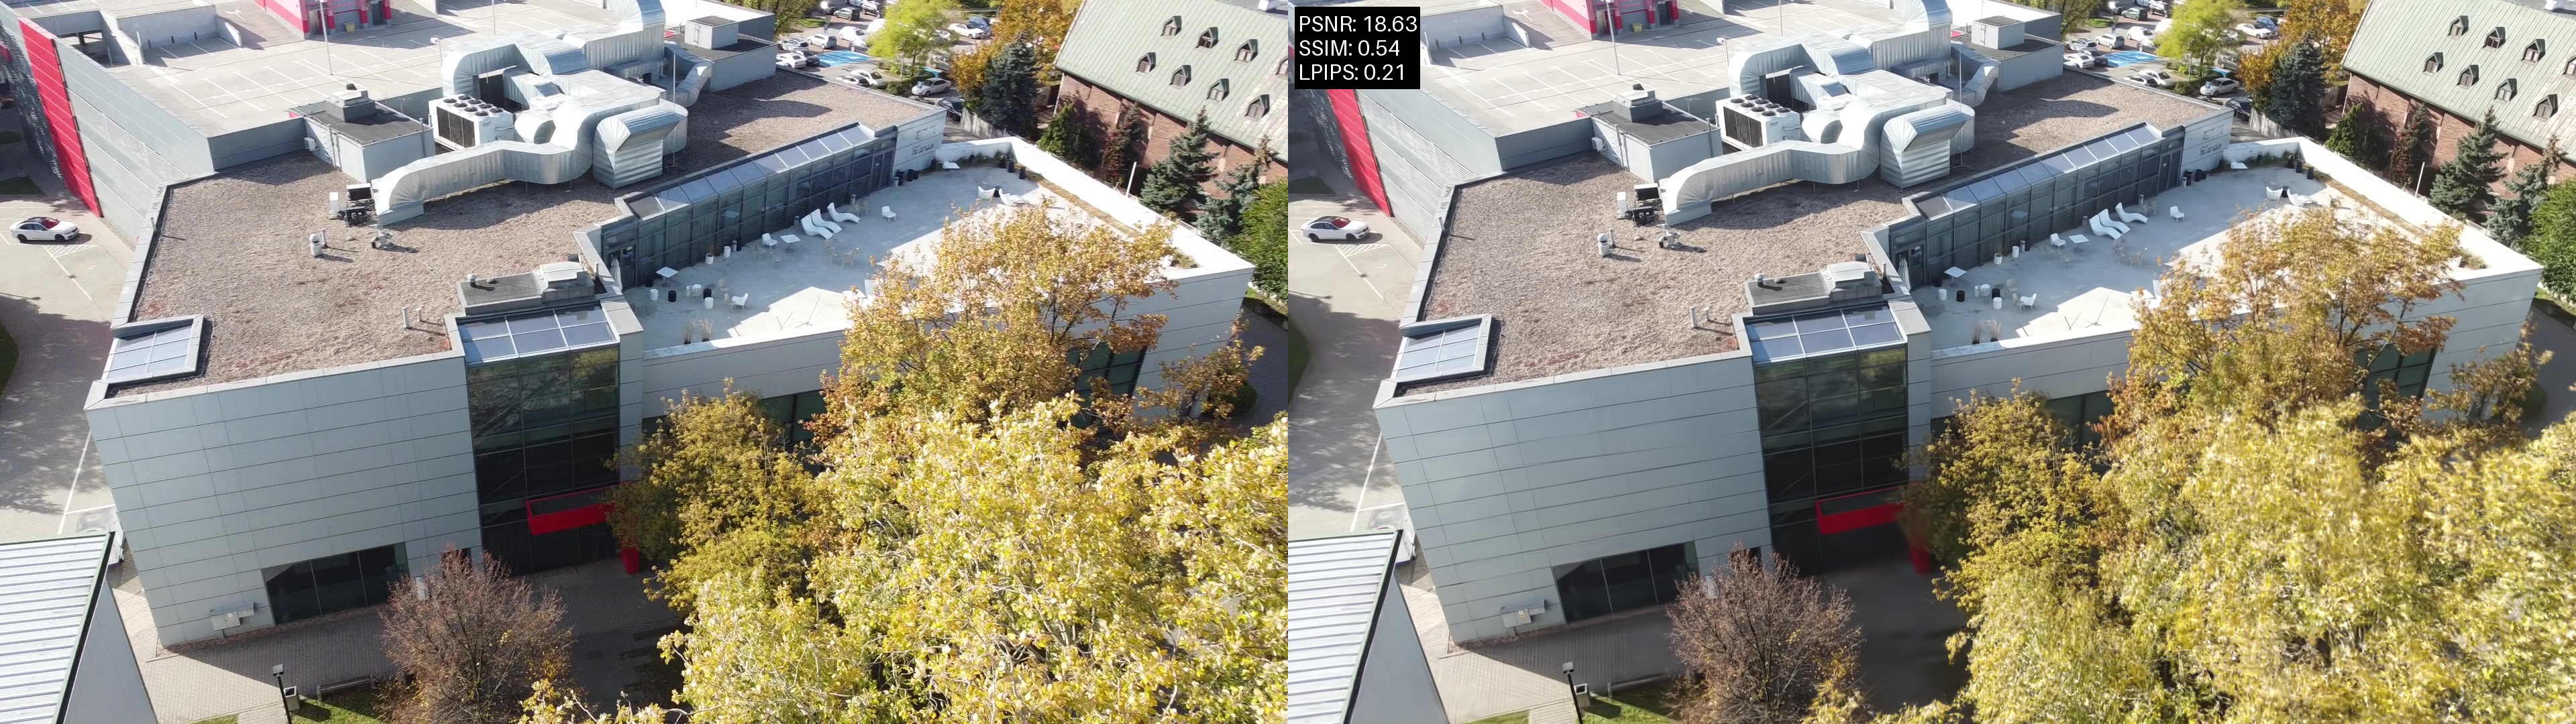
\includegraphics[width=1.0\linewidth]{images/sks_viper_0008.png}
    \caption{Scena SKS}
    \label{fig:sks_gs}
\end{figure}

\begin{figure}[!h]
    \centering
    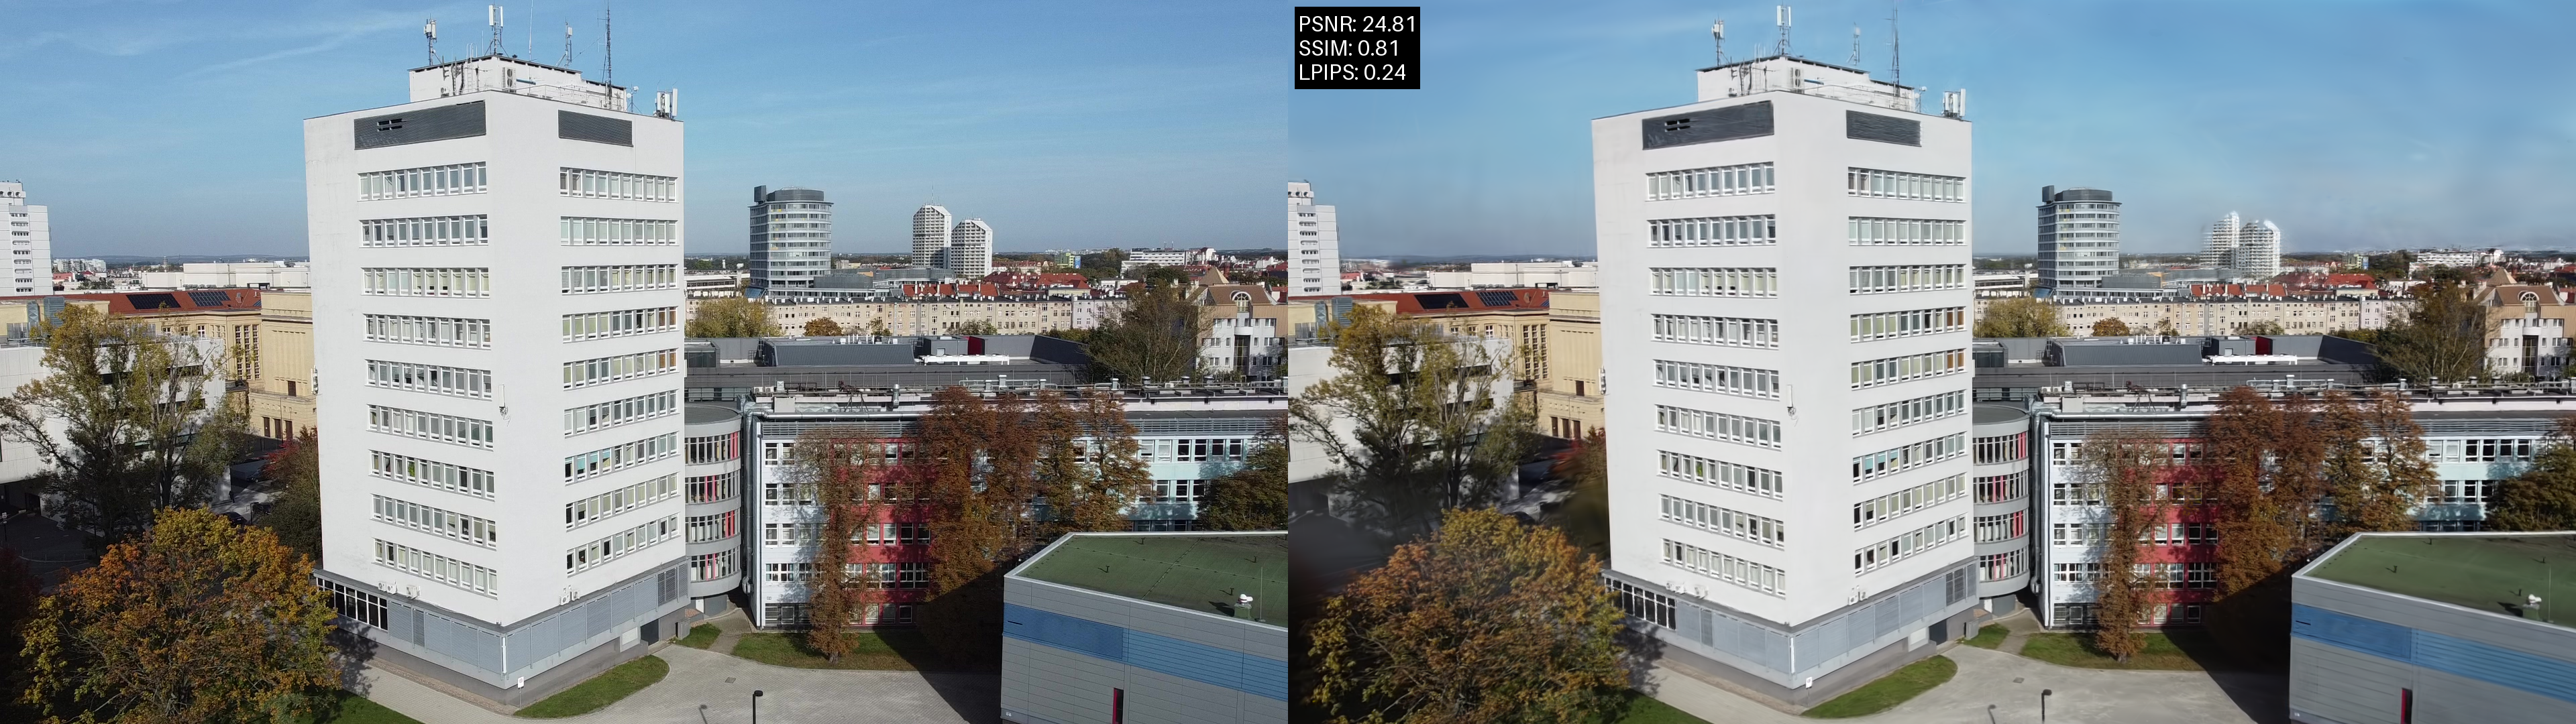
\includegraphics[width=1.0\linewidth]{images/c5_mouse_0001.png}
    \caption{Scena C5}
    \label{fig:c5_gs}
\end{figure}

\begin{figure}[!h]
    \centering
    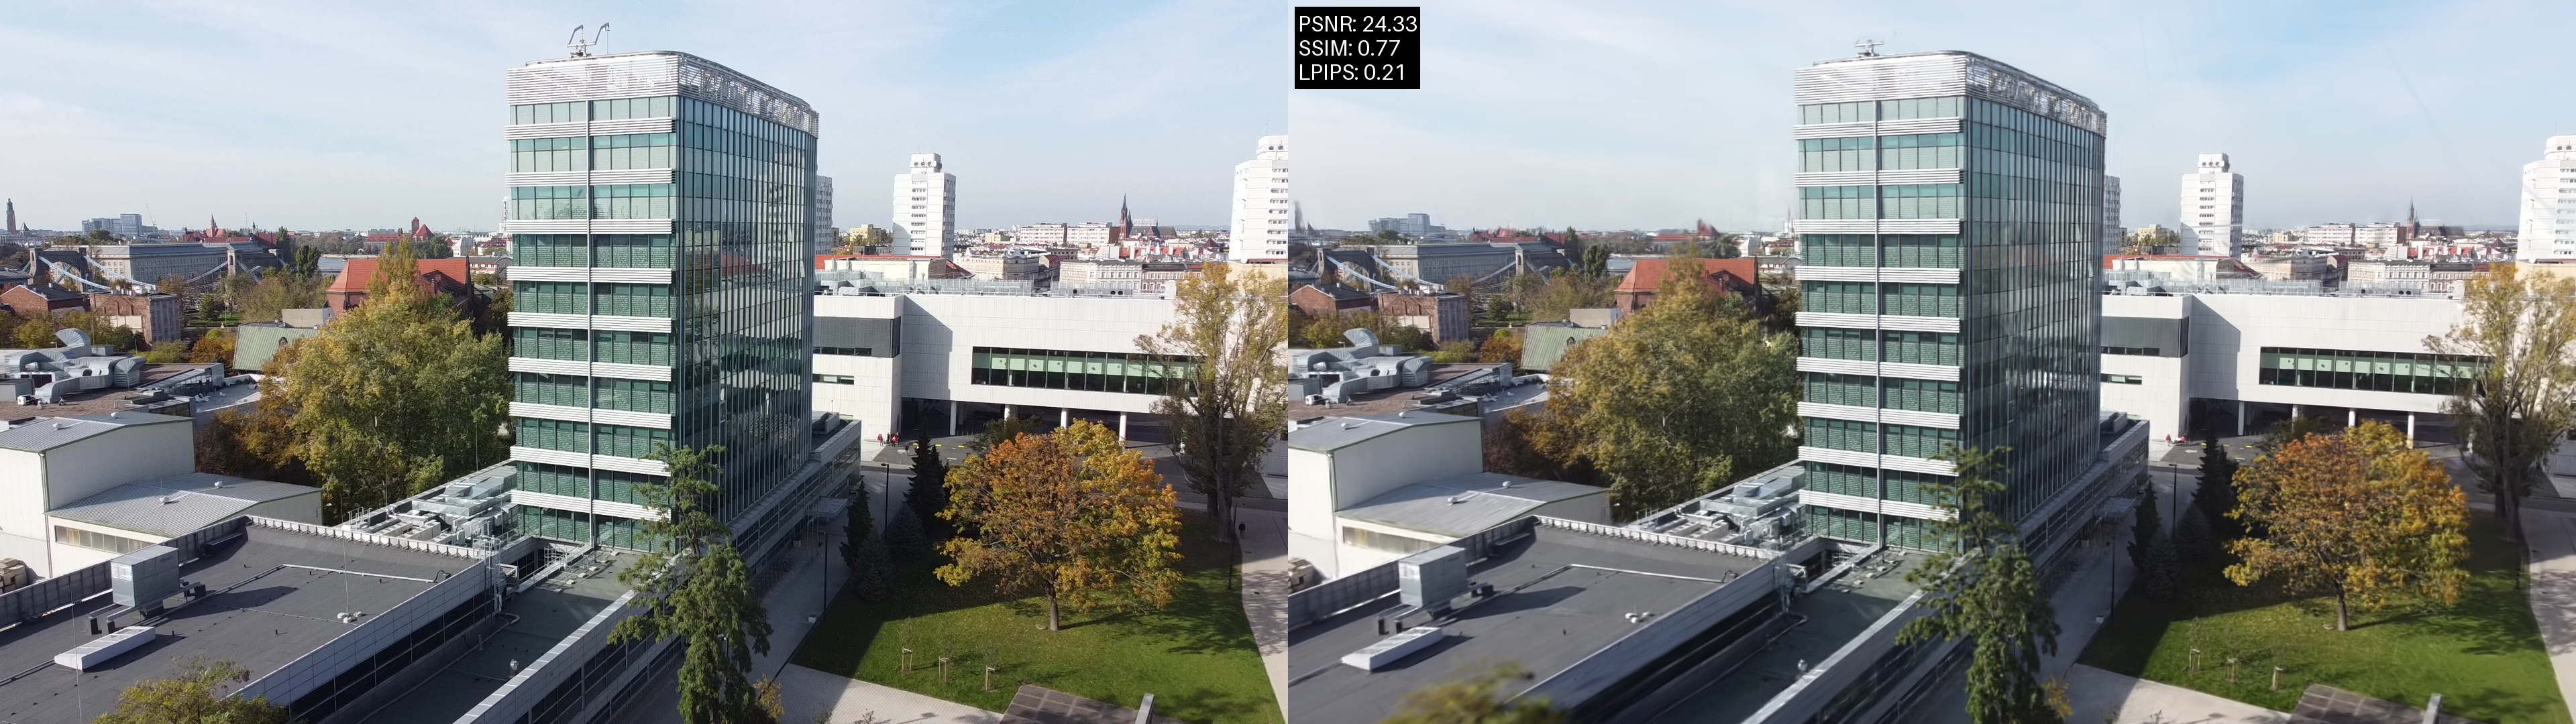
\includegraphics[width=1.0\linewidth]{images/c7_gepard_0006.png}
    \caption{Scena C7}
    \label{fig:c7_gs}
\end{figure}